\documentclass[headings=standardclasses]{scrreprt}

%% Common Packages and Configuration

%% Layout and Style %%
\usepackage{enumitem}
\usepackage{booktabs}
\usepackage{xcolor}
\usepackage{hyperref}
\hypersetup{
  colorlinks=true,
  urlcolor=blue,
  pdfauthor={Severen Redwood},
}

%% Typography %%
\usepackage{fontspec}
\usepackage{microtype}

%% Maths %%
\usepackage{mathtools}
\usepackage{amssymb}
\usepackage{amsthm}
\usepackage[free-standing-units]{siunitx}
\usepackage{unicode-math}

% General
\DeclarePairedDelimiter{\card}{\lvert}{\rvert}
\DeclarePairedDelimiter{\abs}{\lvert}{\rvert}
\DeclarePairedDelimiter{\norm}{\lVert}{\rVert}
\DeclarePairedDelimiter{\ceil}{\lceil}{\rceil}
\DeclarePairedDelimiter{\floor}{\lfloor}{\rfloor}

\newcommand*{\conj}[1]{\overbar{#1}}

% Combinatorics
\newcommand*{\perm}[2]{\prescript{#1}{}P_{#2}}
\newcommand*{\comb}[2]{\prescript{#1}{}C_{#2}}

% Calculus
\DeclareMathOperator{\dif}{d\!}
\newcommand*{\od}[3][]{\frac{\dif{^{#1}}#2}{\dif{#3^{#1}}}}
\newcommand*{\pd}[3][]{\frac{\partial{^{#1}}#2}{\partial{#3^{#1}}}}

% Linear Algebra
\newcommand*{\uvec}[1]{\hat{#1}}
\newcommand*{\ihat}{\uvec{\imath}}
\newcommand*{\jhat}{\uvec{\jmath}}

% Hack in support for augmented matrices into the matrix commands.
\makeatletter
\renewcommand*{\env@matrix}[1][*\c@MaxMatrixCols c]{
  \hskip -\arraycolsep
  \let\@ifnextchar\new@ifnextchar
  \array{#1}
}
\makeatother

% Statistics
\newcommand*{\mean}[1]{\overbar{#1}}

% Theorem-style Environments
\newtheorem{theorem}{Theorem}
\newtheorem{proposition}{Proposition}
\newtheorem{result}{Result}
\theoremstyle{definition}
\newtheorem{definition}{Definition}

%% Language %%
\usepackage{csquotes}
\usepackage{polyglossia}
\setdefaultlanguage[variant=newzealand, ordinalmonthday]{english}


% PDF Metadata
\hypersetup{
  pdftitle={Calculus Notes}
}

% Graphing
\usepackage{tikz}
\usepackage{pgfplots}
\pgfplotsset{compat=1.16}

% Language
\setotherlanguage{greek}
\newfontfamily\greekfont[Script=Greek]{CMU Serif}

\title{Calculus Notes}
\author{Severen Redwood}

\begin{document}

\maketitle

\tableofcontents

\chapter{Limits and Continuity}

A \emph{limit} is the value that a function (or sequence) \enquote{approaches}
as the input (or index) \enquote{approaches} some value. Limits form the
foundation of modern calculus and are used to define continuity, derivatives,
and integrals.

Formally, the limit of a function is written as \[ \lim_{x → c} f(x) = L, \] and
is read as \enquote{the limit of \(f\) of \(x\) as \(x\) approaches \(c\) is
  equal to \(L\)}. Occasionally, a limit may be denoted by a right arrow, as
in \[ f(x) → L \text{ as } x → c. \]

\emph{Continuity} is the property of a function where \emph{sufficiently small
  changes in the input result in sufficiently small changes in the output}. A
function that satisfies this property is \emph{continuous}, and a function that
does not is \emph{discontinuous}.

For example, consider the function \(h(t)\), which describes the height of a
growing flower at time \(t\). This function is continuous. By contrast, if
\(a(t)\) describes the amount of money in a bank account at time \(t\), the
function jumps at each point in time when money is deposited or withdrawn, so
the function \(a\) is discontinuous.

\section{Limits at Infinity}

A \emph{limit at infinity} is the value a function approaches as the input
approaches positive or negative infinity (that is, as the input increases or
decreases without bound). Formally, we write that
\[ \lim_{x → ∞} f(x) = \text{ or } \lim_{x → -∞} f(x) = L. \]

When computing limits at infinity, the following two facts are often useful:

\begin{nfact}
  If \(n ∈ ℚ^{+}\) and \(x ∈ ℝ\), then
  \[ \lim_{x → ∞} \frac{1}{x^{n}} = 0. \]
\end{nfact}

\begin{nfact}
  If \(n ∈ ℚ^{+}\), \(x ∈ ℝ\), and \(x^{n}\) is defined for \(x < 0\), then
  \[ \lim_{x → -∞} \frac{1}{x^{n}} = 0. \]
\end{nfact}

\section{The Squeeze Theorem}

The \emph{squeeze theorem}, or \emph{sandwich theorem}, is a theorem regarding
the limit of a function as it is bounded by two other functions. It is useful
when attempting to determine a limit of a function that is either difficult to
determine or cannot be computed at a given point.

\begin{theorem}[Squeeze Theorem]
  Let \(a\) be a point on the interval \(I\). Let \(g\), \(f\), and \(h\) be
  functions defined at all points on \(I\), except possibly at \(a\) itself.

  Suppose that for every \(x\) in \(I\) not equal to \(a\), we have
  \[ g(x) ≤ f(x) ≤ h(x), \] and also suppose that
  \[ \lim_{x → a } g(x) = \lim_{x → a} h(x) = L. \] Then,
  \[ \lim_{x → a} f(x) = L. \]
\end{theorem}

\begin{figure}[h]
  \centering

  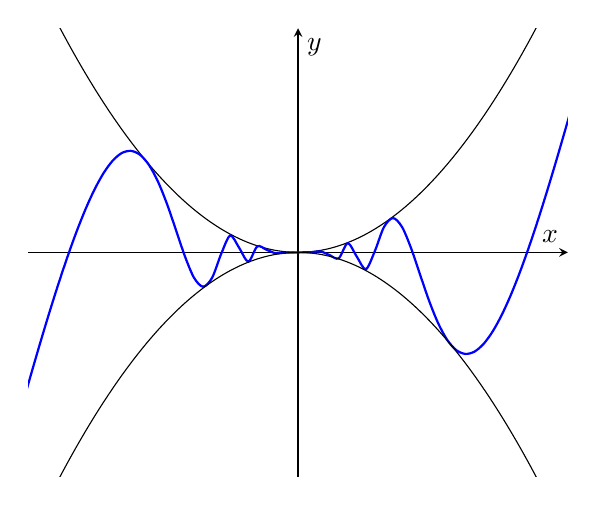
\begin{tikzpicture}
    \begin{axis}[
      xlabel = $x$,
      ylabel = $y$,
      ylabel style = { rotate = -90 },
      xtick = \empty,
      ytick = \empty,
      xmin = -1.5, xmax = 1.5,
      ymin = -1.75, ymax = 1.75,
      axis lines = center,
      samples = 200,
      smooth,
    ]
      \addplot[] {x^2};
      % The frequency is increased to make the illustration look better.
      \addplot[thick, blue] {x^2 * sin(4 * 1/\x r)};
      \addplot[] {-x^2};
    \end{axis}
  \end{tikzpicture}

  \caption{Illustration of \(x^{2} \sin(\frac{1}{x})\) being squeezed as \(x → 0\).}\label{fig:squeeze_theorem}
\end{figure}

\begin{example}
  The limit of \(x^{2} \sin(\frac{1}{x})\) as \(x → 0\) (see
  \autoref{fig:squeeze_theorem}) cannot be determined through direct
  substitution because \(\lim_{x → 0} \sin(\frac{1}{x})\) does not exist.

  However, by the definition of the sine function,
  \[ -1 ≤ \sin(\frac{1}{x}) ≤ 1. \]

  Therefore, it follows that \[ -x^{2} ≤ x^{2} \sin(\frac{1}{x}) ≤ x^{2}. \]

  Since \[ \lim_{x → 0} -x^{2} = \lim_{x → 0} x^{2} = 0, \] by the squeeze
  theorem, \(\lim_{x → 0} [x^{2} \sin(\frac{1}{x})]\) must also be zero.
\end{example}

\section{Continuity at a Point}

A function \(f\) is said to be continuous at \(c\) if it is both defined at
\(c\) and its value at \(c\) equals the limit of \(f\) as \(x\) approaches
\(c\): \[ \lim_{x → c} f(x) = f(c) \]

\chapter{Differentiation}

Differential calculus is the area of calculus that is concerned with the study
of the rates at which quantities change.

The primary object of study in differential calculus is the \emph{derivative of
  a function}, which describes the rate of change of a given function. The
process of finding a derivative is called \emph{differentiation}.

Geometrically, the derivative of a function can be viewed as the function that
gives the slope of a tangent line to the graph of the function at any given
point.

\begin{figure}[h]
  \centering

  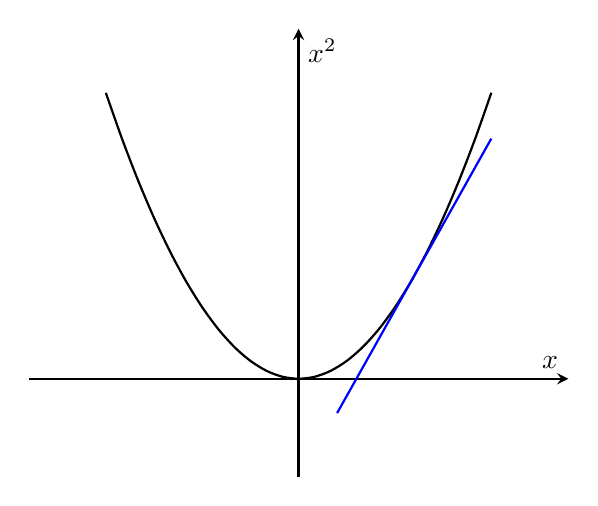
\begin{tikzpicture}
    \begin{axis}[
      xlabel = $x$,
      ylabel = $x^{2}$,
      ylabel style = { rotate = -90 },
      xtick = \empty,
      ytick = \empty,
      axis lines = center,
      enlargelimits = 0.2,
      smooth,
      thick,
    ]
      \addplot[] {x^2};
      \addplot[color = blue] coordinates {(1, -3) (5, 21)};
    \end{axis}
  \end{tikzpicture}

  \caption{Graph of \(x^{2}\) and a tangent line at \(x = 3\).}
\end{figure}

\section{Notation}

Differential calculus has no single uniform notation for differentiation.
Several different notations for the derivative of a function or variable have
been proposed by different mathematicians, the most common of which are
Langrange's\footnote{Joseph Lewis Lagrange was an Italian Enlightenment Era
  mathematician and astronomer.} and Leibniz's\footnote{Gottfried Wilhelm von
  Leibniz was a German Enlightenment Era polymath most notably known as (one of)
  the inventors of differential and integral calculus.}.

While this may appear to be a mess at first, the usefulness of each notation
varies with context, as it is sometimes advantageous to use more than one
notation in a given context.

\subsection{Lagrange's Notation}

Lagrange's notation makes use of a prime mark to denote a derivative.

For example, if \(f\) is a function, then its derivative evaluated at \(x\) is
written as \(f'(x)\) and pronounced as \enquote{f prime of x}. Similarly, if a
function is written in the form \(y = f(x)\), the derivative can be expressed as
\(y'\).

Higher derivatives are indicated with additional prime marks, as in \(f''\) for
the second derivative and \(f'''\) for the third derivative. Since this quickly
becomes unwieldy, some authors continue by either employing Roman numerals
(\(f^{\mathrm{IV}}\)) or Arabic numerals in brackets (\(f^{(4)}\)).

\subsection{Leibniz's Notation}

Leibniz's notation makes use of\ldots

\[ \frac{\dif y}{\dif x} \]

\subsection{Newton's Notation}

Newton's notation makes use of a dot to denote a derivative.

For example, if \(f\) is a function, then its derivative evaluated at \(x\) is
written as \(\dot f(x)\) and pronounced as \enquote{f dot of x}. Similarly, if a
function is written in the form \(y = f(x)\), the derivative can be expressed as
\(\dot y\).

Newton's notation is mostly used in physics and other sciences where calculus is
applied in a real-world context, and consequently is not seen often in pure
mathematics.

\section{Implicit Differentiation}

\emph{Implicit differentiation} is an application of the chain rule to
\emph{implicit functions} in order to make such functions easier (or, in some
cases, possible at all) to differentiate.

\begin{definition}[Implicit Function]
  An \emph{implicit equation} is a relation of the form
  \[ R(x_{1}, \dots, x_{n}) = 0, \] where \(R\) is a function of several
  variables.

  An \emph{implicit function} is a function that is defined implicitly by an
  implicit equation, by associating one of the variables (the value) with the
  others (the arguments).
\end{definition}

\begin{example}
  The implicit equation of the unit circle is \[ x^{2} + y^{2} - 1 = 0. \]
  Therefore, an implicit function for \(y\) in the context of the unit circle is
  defined implicitly by \(x^{2} + {y(x)}^{2} - 1 = 0\). With this particular
  equation, we can rewrite it in the form \[ y = ±\sqrt{1 - x^{2}}, \] which
  \emph{explicitly} defines the two functions that were previously defined
  implicitly.
\end{example}

Implicit differentiation is a useful tool because not every implicit equation,
and therefore not every implicit function, can be made explicit and
differentiated using normal means. For example, no amount of algebra will yield
an explicit solution to the equation \(y^{5} + 2y^{4} - 7y^{3} + 3y^{2} - 6y - x
= 0\). In this situation, implicit differentiation is required.

In implicit differentiation, we differentiate each side of an equation with two
variables (usually \(x\) and \(y\)) by treating one of the variables as a
function of the other.

\end{document}
